\documentclass{article}
\usepackage[margin=1in]{geometry}
\usepackage{amsmath}
\usepackage{graphicx}
\usepackage{float}
\usepackage{listings}
\usepackage{subcaption}
\usepackage{changepage}
\usepackage{hyperref}

\title{Report: Distributed Systems Homework 2}
\author{Moida Praneeth Jain (2022101093), Richa Verma (2024202010)}
\date{\today}

\begin{document}

\maketitle

\section{MPI Sparse Matrix Row-Row Multiplication}

\subsection{Problem Understanding}
The goal of this project is to implement a parallel sparse matrix-matrix multiplication (SpGEMM) algorithm using the Message Passing Interface (MPI). The multiplication computes $C = A \times B$, where A and B are large, sparse matrices. A row-oriented approach is used, where rows of matrix A are distributed among processes to compute corresponding rows of the result matrix C. The implementation is efficient, scaling with the number of available processor cores and handling the sparse data structures effectively.

\subsection{System Setup}
\begin{itemize}
    \item \textbf{Programming Language:} C++ (Standard: C++17)
    \item \textbf{Parallelism Framework:} OpenMPI
    \item \textbf{Cluster Configuration:} The performance analysis was conducted on the SLURM cluster, utilizing a single node with 32 cores and 93Gi RAM.
    \item \textbf{Compilation:} The code was compiled using \texttt{mpic++} with \texttt{-O3} and \texttt{-march=native} flags for performance optimization.
\end{itemize}

\subsection{Design and Implementation}
The implementation follows a primary-worker (master-slave) pattern, where rank 0 is the primary process responsible for data distribution and result aggregation.

\subsubsection{Parallelization Strategy}
The core strategy is to parallelize the computation of the output matrix C by distributing the rows of matrix A among the available MPI processes. Each process $p$ is responsible for calculating a subset of rows of C, denoted $C_p$, by multiplying its assigned rows of A, denoted $A_p$, with the entire matrix B.

\subsubsection{Data Distribution}
\begin{enumerate}
    \item \textbf{Initial Read:} The primary process (rank 0) reads the entire sparse matrices A and B from an input file. Matrix B is read into a memory-efficient, CSR-like format (using three separate vectors for row pointers, column indices, and values).
    \item \textbf{Matrix B Broadcast:} The complete matrix B is broadcast to all worker processes using \texttt{MPI\_Bcast}. This is necessary because every process needs full access to B to compute its assigned rows of C.
    \item \textbf{Matrix A Distribution (Dynamic Load Balancing):} To distribute the rows of matrix A, a dynamic load balancing scheme is used. Rank 0 iterates through each row of A and assigns it to the worker process that currently has the minimum accumulated workload. The workload is estimated by the total number of non-zero elements in the rows assigned to that worker so far. This helps to evenly distribute the computational effort, especially when the rows of A have varying sparsity. The row data is then transmitted to the respective workers using a combination of \texttt{MPI\_Scatter} (for counts) and point-to-point \texttt{MPI\_Send}/\texttt{MPI\_Recv} calls.
\end{enumerate}

\subsubsection{Communication Patterns}
\begin{itemize}
    \item \texttt{MPI\_Bcast}: Used to efficiently distribute matrix dimensions (N, M, P) and the entirety of matrix B to all processes.
    \item \texttt{MPI\_Scatter} and \texttt{MPI\_Send}/\texttt{MPI\_Recv}: Used in combination to distribute the rows of matrix A from rank 0 to the workers.
    \item \texttt{MPI\_Reduce}: Used at the end of the computation to find the maximum execution time among all processes for accurate benchmarking.
    \item \texttt{MPI\_Send}/\texttt{MPI\_Recv} (for results): After computing their local results, worker processes send their calculated rows of C back to the primary process (rank 0), which assembles the final output matrix.
\end{itemize}

\subsubsection{Computational Optimization}
A hybrid approach is used for the inner multiplication loop. Based on an estimated number of floating-point operations, the algorithm chooses between two accumulator strategies:
\begin{itemize}
    \item \textbf{Hash Map (\texttt{std::unordered\_map}):} For highly sparse result rows, a hash map is used to accumulate the values for each column index. This is memory-efficient when the number of non-zero elements in the output row is small.
    \item \textbf{Dense Vector (\texttt{std::vector}):} If the estimated number of operations exceeds a threshold (\texttt{DENSE\_THR}), a dense vector is used as an accumulator. This is faster for denser output rows as it avoids the overhead of hash collisions and lookups.
\end{itemize}

\subsection{Execution Details}
\begin{itemize}
    \item \textbf{Compilation Command:}
    \begin{lstlisting}[language=bash]
mpic++ -O3 -march=native -std=c++17 main.cpp -o sparse_matmul_cpp
    \end{lstlisting}
    \item \textbf{Execution Command:}
    \begin{lstlisting}[language=bash]
mpirun -n <num_procs> --oversubscribe ./sparse_matmul_cpp <input_file>
    \end{lstlisting}
\end{itemize}

\subsection{Performance Evaluation}
The performance was benchmarked by running the program with varying numbers of processor cores on matrices of different sizes. The following plots were generated from the \texttt{slurm\_scaling\_results.csv} data.

\begin{figure}[H]
  \centering
  
  \begin{subfigure}[b]{0.7\textwidth}
    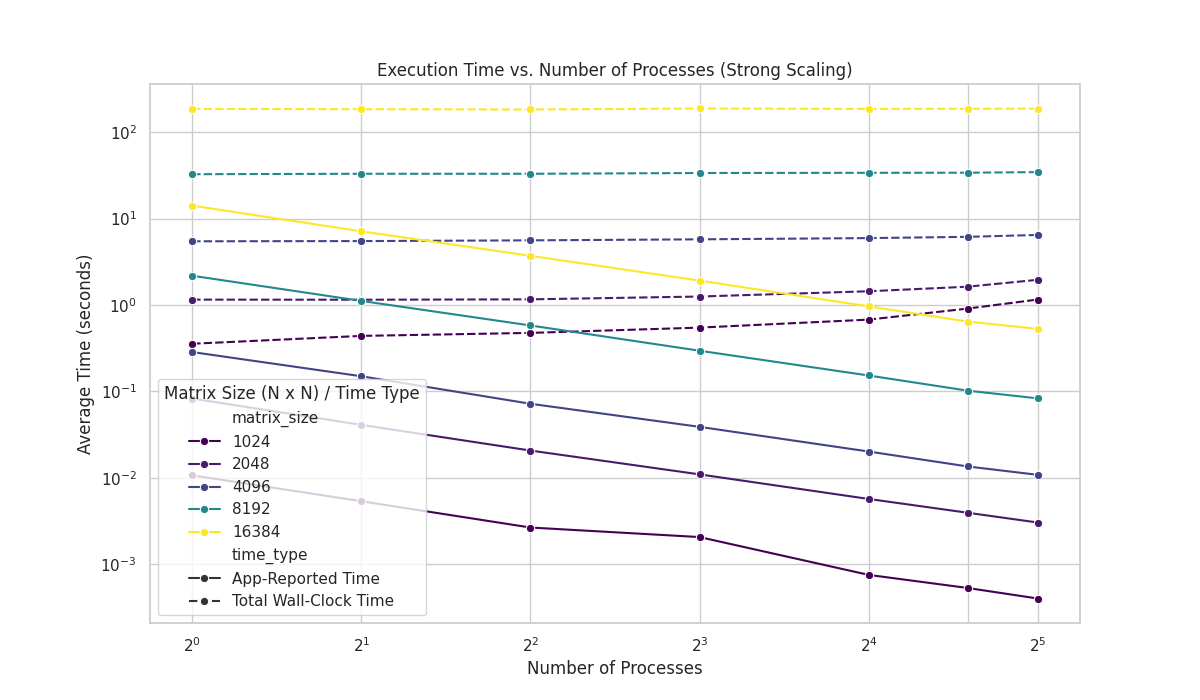
\includegraphics[width=\linewidth]{sparse_matmul_cpp/plots/1_execution_time_comparison.png}
    \caption{Execution Time}
    \label{fig:exec_time}
  \end{subfigure}

  \vspace{1em}
  \begin{subfigure}[b]{0.4\textwidth}
    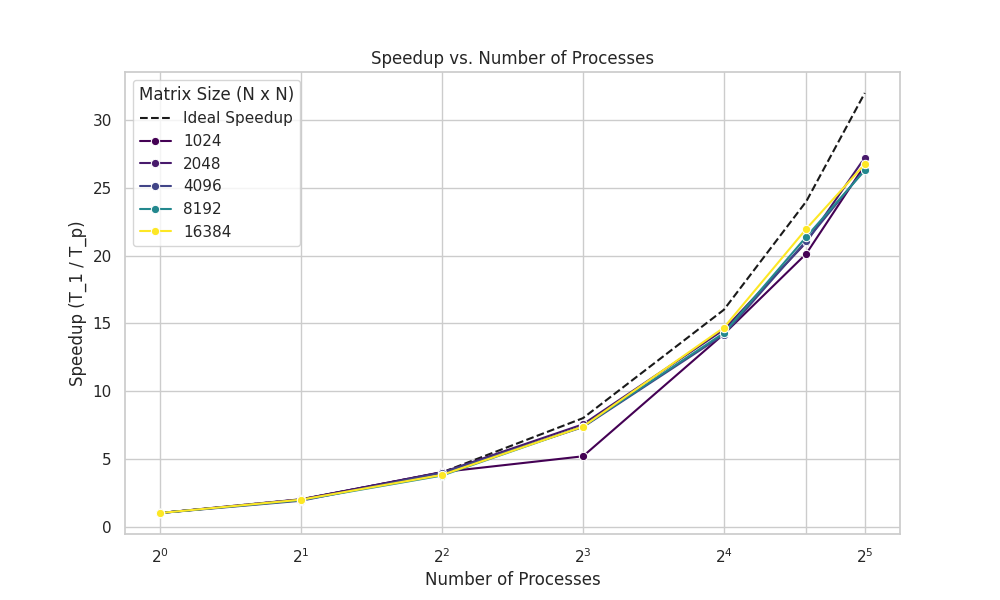
\includegraphics[width=\linewidth]{sparse_matmul_cpp/plots/2_speedup.png}
    \caption{Speedup}
    \label{fig:speedup}
  \end{subfigure}
  \hfill
  \begin{subfigure}[b]{0.4\textwidth}
    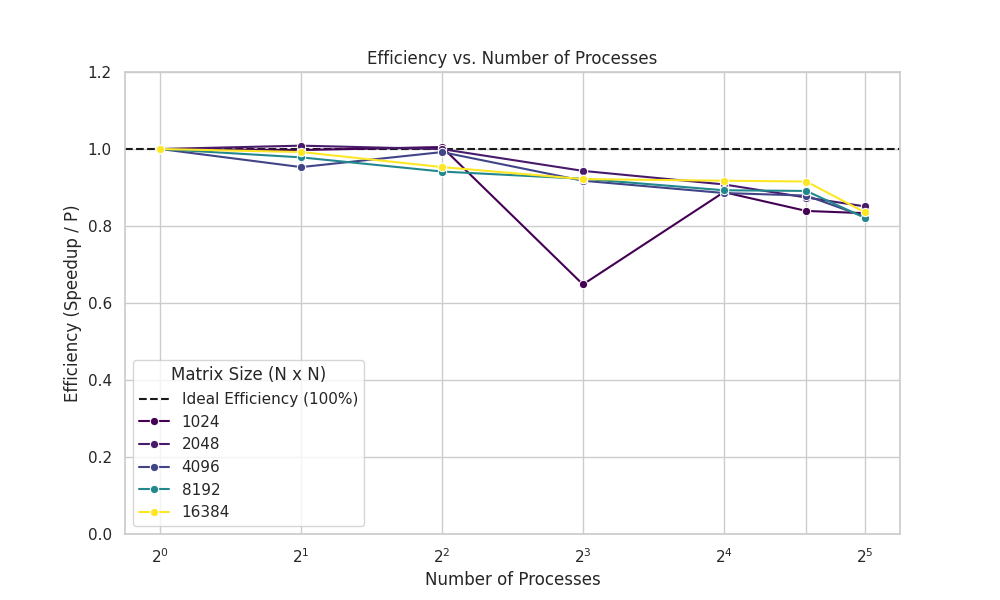
\includegraphics[width=\linewidth]{sparse_matmul_cpp/plots/3_efficiency.png}
    \caption{Efficiency}
    \label{fig:efficiency}
  \end{subfigure}

  \caption{Scaling Analysis: (a) Execution time (b) Speedup (c) Efficiency vs. number of cores}
  \label{fig:perf_metrics}
\end{figure}

\begin{figure}[H]
    \centering
    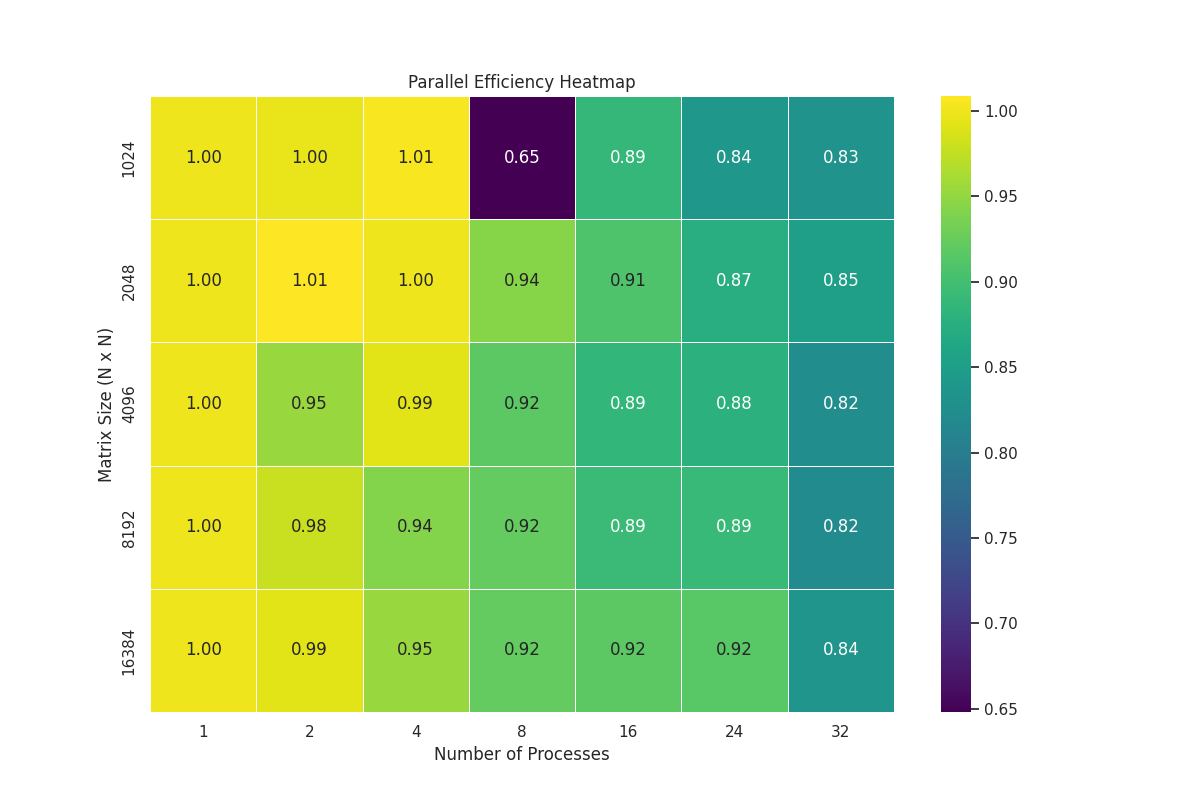
\includegraphics[width=0.6\textwidth]{sparse_matmul_cpp/plots/5_efficiency_heatmap.png}
    \caption{Efficiency Heatmap. This heatmap visualizes the parallel efficiency across different matrix sizes and core counts.}
\end{figure}

\subsection{Challenges and Limitations}
\begin{itemize}
    \item \textbf{Rank 0 Bottleneck:} The primary process (rank 0) is responsible for all initial I/O and data distribution. This centralized approach can become a bottleneck, as all other processes must wait for rank 0 to finish reading and sending data before computation can begin.
    \item \textbf{Memory Usage:} Broadcasting the entire matrix B to all processes consumes a significant amount of memory on each node, limiting the maximum problem size that can be solved.
    \item \textbf{Result Aggregation:} All result rows are sent back to rank 0. For very large matrices, this can overwhelm the memory of the primary process and create a communication bottleneck at the end of the computation.
\end{itemize}

\subsection{Conclusion and Future Work}
The MPI-based sparse matrix multiplication implementation successfully parallelizes the computation, achieving good speedup and scalability. The dynamic load balancing scheme for distributing rows of matrix A is effective.

Future improvements could include:
\begin{itemize}
    \item Implementing parallel I/O to remove the rank 0 bottleneck for data loading.
    \item Exploring a 2D decomposition of the matrix to partition both matrix A and B, reducing the memory footprint on each node.
    \item Using a tree-based communication pattern for aggregating results instead of sending everything directly to rank 0.
\end{itemize}

\section{MapReduce K-Means Clustering}

\subsection{Problem Understanding}
This project implements the K-Means clustering algorithm using a MapReduce paradigm simulated with MPI. K-Means is an iterative algorithm that partitions a dataset into K distinct, non-overlapping clusters. The MapReduce model is a natural fit for this: the \texttt{Map} phase assigns each data point to its nearest cluster centroid, and the \texttt{Reduce} phase recalculates the new centroids based on the mean of the points assigned to them.

\subsection{System Setup}
\begin{itemize}
    \item \textbf{Programming Language:} Rust
    \item \textbf{Parallelism Framework:} OpenMPI (used to simulate the MapReduce model)
    \item \textbf{Cluster Configuration:} The performance analysis was conducted on the SLURM cluster, utilizing a single node with 32 cores and 93Gi RAM.
    \item \textbf{Build System:} Cargo, with the project built in release mode for optimization.
\end{itemize}

\subsection{Design and Implementation}
The implementation simulates the MapReduce pattern over several iterations until the cluster centroids converge or a maximum number of iterations is reached. Each iteration consists of a Map phase and a Reduce phase, orchestrated by MPI.
\begin{itemize}
    \item \textbf{Map Phase:} Each worker process receives a subset of the total data points. In the \texttt{map\_and\_combine} function, each worker iterates through its local points, assigning each one to the nearest of the current K centroids. Most importantly, this phase includes a "local combine" optimization: each worker pre-aggregates the sum of coordinates and the count of points for each cluster among its local data. This reduces the amount of data that needs to be communicated during the reduce phase.
    \item \textbf{Reduce Phase:} The root process (rank 0) acts as the reducer. It receives the local sums and counts from all worker processes using an \texttt{MPI\_Reduce} operation with a \texttt{SUM} operator. It then computes the new global centroids by dividing the global sums by the global counts.
\end{itemize}

\subsubsection{Data Distribution}
\begin{enumerate}
    \item \textbf{Initial Data Scatter:} At the start, the root process reads the complete set of data points and scatters disjoint subsets to all worker processes using \texttt{scatter\_into\_root}.
    \item \textbf{Centroid Broadcast:} In each iteration, after the root process computes the new centroids, it broadcasts them to all worker processes using \texttt{MPI\_Bcast}. This ensures all workers have the latest centroids for the next map phase.
\end{enumerate}

\subsubsection{Communication Patterns}
\begin{itemize}
    \item \texttt{MPI\_Scatter}: Used once at the beginning to distribute the input data points.
    \item \texttt{MPI\_Bcast}: Used in every iteration to broadcast the updated centroids and the final convergence status.
    \item \texttt{MPI\_Reduce}: Used in every iteration to aggregate local sums and counts from workers to the root process to compute new centroids.
    \item \texttt{MPI\_Barrier}: Used for synchronization between phases to ensure accurate timing measurements for the map and reduce steps.
\end{itemize}

\subsection{Execution Details}
\begin{itemize}
    \item \textbf{Build Command:}
    \begin{lstlisting}[language=bash]
cargo build --release
    \end{lstlisting}
    \item \textbf{Execution Command (from \texttt{run\_km\_mapreduce.sh}):}
    \begin{lstlisting}[language=bash]
mpirun -np <num_procs> target/release/kmeans_mapreduce <args>
    \end{lstlisting}
    The arguments specify the number of centers, input files, max iterations, and output directory.
\end{itemize}

\subsection{Performance Evaluation}
Performance was evaluated to show how the implementation scales with the number of cores.

\begin{figure}[H]
    \begin{adjustwidth}{-2cm}{-2cm}
    \centering
    
    \begin{subfigure}[b]{0.6\textwidth}
        
\includegraphics[width=\linewidth]{kmeans_mapreduce/slurm_plots/combined_time_vs_cores.png}
        \caption{Execution Time vs. Number of Cores}
        \label{fig:kmeans_time}
    \end{subfigure}%
    \begin{subfigure}[b]{0.6\textwidth}
        
\includegraphics[width=\linewidth]{kmeans_mapreduce/slurm_plots/combined_speedup_vs_cores.png}
        \caption{Speedup vs. Number of Cores}
        \label{fig:kmeans_speedup}
    \end{subfigure}

    \vspace{0.5em}
    \begin{subfigure}[b]{0.6\textwidth}
        
\includegraphics[width=\linewidth]{kmeans_mapreduce/slurm_plots/combined_efficiency_vs_cores.png}
        \caption{Efficiency vs. Number of Cores}
        \label{fig:kmeans_efficiency}
    \end{subfigure}%
    \begin{subfigure}[b]{0.6\textwidth}
        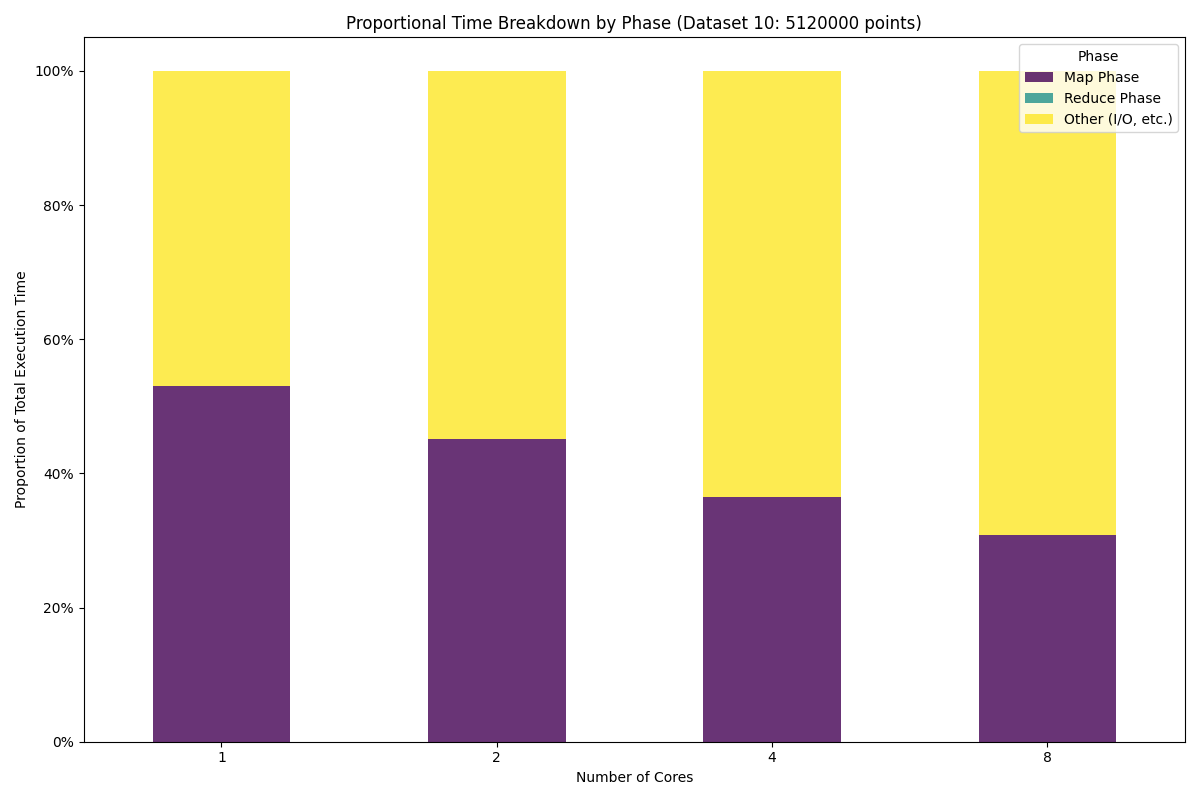
\includegraphics[width=\linewidth]{kmeans_mapreduce/plots/proportional_breakdown_dataset_10.png}
        \caption{Proportional Breakdown for Dataset 10}
        \label{fig:kmeans_breakdown}
    \end{subfigure}
\end{adjustwidth}
    \caption{Performance Analysis: (a) Clear reduction in execution time with increasing cores. (b) Near-linear speedup at lower core counts with diminishing returns due to communication overhead. (c) High parallel efficiency that decreases with more cores. (d) Time distribution across map, reduce, and other phases for a large dataset.}
    \label{fig:kmeans_perf}
\end{figure}

\begin{figure}[H]
    \centering
    
\includegraphics[width=0.8\textwidth]{kmeans_mapreduce/slurm_plots/3d_performance_surface.png}
    \caption{3D Performance Surface. This plot shows the relationship between the number of cores, the size of the dataset, and the execution time.}
\end{figure}


\subsection{Challenges and Limitations}
\begin{itemize}
    \item \textbf{Iterative Communication Overhead:} The algorithm requires a broadcast and a reduce operation in every single iteration. For datasets that require many iterations to converge, this communication can become a significant performance bottleneck, limiting scalability.
    \item \textbf{Root Process Workload:} The root process is solely responsible for computing the new centroids and checking for convergence. While not computationally intensive, this serial step is part of Amdahl\'s law and limits overall speedup.
    \item \textbf{Memory Constraints:} The initial scatter requires the root process to first load the entire dataset into memory, which can be a limitation for extremely large datasets.
\end{itemize}

\subsection{Conclusion and Future Work}
The K-Means algorithm was successfully implemented using an MPI-based MapReduce model in Rust. The use of a local combiner significantly optimizes the reduce step, and the overall implementation shows good scalability.

Potential future work includes:
\begin{itemize}
    \item Implementing a tree-based reduction (\texttt{MPI\_Allreduce}) so that all processes have the new centroids without waiting for a broadcast from the root, potentially reducing communication latency.
    \item Exploring parallel I/O to allow all processes to read their portion of the data directly from the filesystem.
    \item Implementing a more advanced version of K-Means, such as K-Means++, to improve the quality of the initial centroid selection.
\end{itemize}

\section{gRPC Matrix Calculation Server}

\subsection{Problem Understanding}
This project is a gRPC server, written in Rust, that provides a service for matrix operations. The server is designed to allow a client to build a square matrix by sending its rows one by one via a stream. Once the matrix is complete, the server pre-computes and caches its rank and determinant. Subsequent client queries for these properties are answered using the cached values, ensuring high performance for repeated queries.

\subsection{System Setup}
\begin{itemize}
    \item \textbf{Programming Language:} Rust
    \item \textbf{Frameworks:} \texttt{tonic} for gRPC, \texttt{tokio} for asynchronous runtime.
    \item \textbf{Protocol:} gRPC with Protocol Buffers.
    \item \textbf{Architecture:} A single-server, multi-client model. The server is asynchronous and can handle multiple client connections concurrently.
\end{itemize}

\subsection{Design and Implementation}
The server exposes a \texttt{MatrixService} with two RPC methods: \texttt{Interact} and \texttt{Reset}.

\subsubsection{Concurrency and State Management}
The server needs to manage a shared state (the matrix being built, its dimensions, and cached results) across multiple concurrent client requests. This is achieved using an \texttt{Arc<Mutex<AppState>>}.
\begin{itemize}
    \item \textbf{\texttt{Arc} (Atomically Referenced Counter):} Allows multiple threads (or in this case, asynchronous tasks) to safely share ownership of the application state.
    \item \textbf{\texttt{Mutex} (Mutual Exclusion):} Ensures that only one task can access and modify the \texttt{AppState} at any given time. This prevents race conditions, such as two clients trying to add rows to the matrix simultaneously.
\end{itemize}

\subsubsection{Communication Patterns}
\begin{itemize}
    \item \textbf{Bidirectional Streaming (\texttt{Interact} RPC):} The primary interaction happens through this stream. The client can send a stream of \texttt{ClientRequest} messages (e.g., \texttt{Row} commands). The server processes these and can send back a stream of \texttt{ServerResponse} messages (e.g., query results or errors). This is highly efficient as it uses a single, long-lived HTTP/2 connection.
    \item \textbf{Unary RPC (\texttt{Reset}):} A simple request-response method to clear the server\'s state and allow for the construction of a new matrix.
\end{itemize}

\subsubsection{Performance Optimization: Caching}
The core performance feature is the caching mechanism.
\begin{enumerate}
    \item The server determines the matrix dimension from the first row it receives.
    \item It accepts rows until the number of rows equals the dimension, signifying a complete square matrix.
    \item At this exact moment, it triggers the computation of the matrix\'s rank (via Gaussian elimination) and determinant.
    \item These values are stored in \texttt{cached\_rank} and \texttt{cached\_determinant} within the \texttt{AppState}.
    \item All subsequent queries for rank or determinant are answered instantly from these cached values, avoiding any redundant, expensive calculations. The matrix itself is effectively immutable until a \texttt{Reset} is called.
\end{enumerate}

\subsection{Execution Details}
\begin{itemize}
    \item \textbf{Run Server Command:}
    \begin{lstlisting}[language=bash]
cargo run --bin server
    \end{lstlisting}
    \item \textbf{Run Client Command:}
    \begin{lstlisting}[language=bash]
cargo run --bin client
    \end{lstlisting}
\end{itemize}

\subsection{Performance Evaluation}
\begin{itemize}
    \item a) No empirical performance data (e.g., latency benchmarks, throughput tests) was generated for this project.
    \item b) The design is nevertheless performance-oriented. The primary performance gain comes from the \textbf{calculate-once, query-many} caching strategy. The cost of calculating the determinant and rank is paid only a single time when the matrix is finalized. All subsequent queries are O(1) lookups. The use of \texttt{tokio} and asynchronous gRPC allows the server to handle many concurrent client connections with high efficiency, as it does not block threads waiting for I/O.
\end{itemize}

\subsection{Challenges and Limitations}
\begin{itemize}
    \item \textbf{Mutex Contention:} The use of a single \texttt{Mutex} to protect the entire application state is simple and safe, but it can become a performance bottleneck under high load. If many clients attempt to send rows or queries simultaneously, they will be serialized, waiting to acquire the lock.
    \item \textbf{Custom Math Implementation:} The matrix operations (\texttt{calculate\_rank}, \texttt{calculate\_determinant}) are custom implementations. While functional, they may not be as numerically stable or as highly optimized as those found in dedicated linear algebra libraries like BLAS or LAPACK.
    \item \textbf{No Partial Results:} The design is rigid: queries can only be answered once the \textit{entire} matrix is built. It does not support queries on partially constructed matrices.
\end{itemize}

\subsection{Conclusion and Future Work}
The gRPC server provides a robust and efficient service for its specific use case: building a matrix and repeatedly querying its properties. The use of bidirectional streaming and a caching layer are key strengths of the design.

Future work could involve:
\begin{itemize}
    \item \textbf{Improved Concurrency:} Replacing the single \texttt{Mutex} with more granular locking (e.g., \texttt{RwLock} to allow concurrent reads) could improve performance for query-heavy workloads.
    \item \textbf{Production-Grade Math Library:} Integrating a battle-tested linear algebra library could improve the performance and numerical stability of the rank and determinant calculations.
    \item \textbf{Benchmarking:} Developing a proper benchmarking suite to measure request latency, throughput, and scalability under various client loads.
\end{itemize}

\end{document}